\documentclass[11pt,a4paper,twocolumn]{article}
\title{A study of machine learning approaches\\to cross-language code clone detection}
\date{January 26, 2018}
\author{Daniel Perez}
\usepackage[left=0.9cm,right=0.9cm,top=1.2cm,bottom=1.5cm]{geometry}
\usepackage{titling}
\usepackage{graphicx}
\usepackage{amsmath}
\usepackage{amsfonts}
\usepackage{fontspec}
\usepackage{titlesec}
\setlength{\droptitle}{-5em}
\posttitle{\end{center}\vspace{-1.5em}}
\postauthor{\end{tabular}\end{center}\vspace{-2em}}
\postdate{\end{center}\vspace{-1em}}
\titlespacing*{\section}
{0pt}{1.5ex plus 0ex minus .2ex}{1ex plus .2ex}
\titlespacing*{\subsection}
{0pt}{1ex plus 1ex minus .2ex}{1ex plus .2ex}
\usepackage{amsmath}
\makeatletter
\g@addto@macro\normalsize{%
  \setlength\abovedisplayskip{5pt}
  \setlength\belowdisplayskip{5pt}
  \setlength\abovedisplayshortskip{40pt}
  \setlength\belowdisplayshortskip{40pt}
}
\makeatother
%
\begin{document}
\maketitle
\section*{Abstract}
While clone detection across programs written in the same programming language
has been studied extensively in the literature, the task of detecting clones
across multiple programming languages is not covered as well, and approaches
based on comparison cannot be directly applied.
In this thesis, we present a clone detection method based on supervised
machine learning able to detect clone across programming languages.
Our method uses an unsupervised learning approach to learn token-level vector
representations and an LSTM-based neural network to predict if two code
fragments are clones. To train our network, we present a cross-language code
clone dataset --- which is to the best of our knowledge the first of its kind
--- containing more than 50000 code fragments written in Python and Java.
We show that our method is able to detect code clones between Python and Java.
We also compare our method to state-of-the-art tools in single-language clone
detection and show we achieve better F1-score.
\section{Background}
Code clone detection is the task of detecting similar piece of codes inside or
across software projects. Literature has mostly focused on detecting
clones for code fragments written in the same programming
language~\cite{Roy07asurvey}.
However, it is very common for large systems to be divided in
smaller sub-systems implemented using different programming languages. Being
able to detect code clones across these sub-systems could help finding
refactoring opportunities, but it requires detecting code clones across
programming languages.

Although some approaches to cross-language clone detection such as
tree comparison based approach using a common intermediate
representation~\cite{DBLP:conf/seke/KraftBS08} have been proposed, to the best
of our knowledge no approach using only source code and not relying on
similarity between input programming languages currently exists.

In this paper, we propose a supervised learning approach to detect
cross-language clone detection and provide a dataset to train our model.
The implementation is partly available on GitHub\footnote{https://github.com/tuvistavie/bigcode-tools}.
\section{Our proposal}
\subsection{Overview}
Our method is divided into two main parts: learning a token-level vector
representation for each language, and learning a function to classify
code clones.
\subsection{\label{ssec:token-representation}Token-level vector representation}
To learn token-level representation, we based our method on the skipgram
algorithm~\cite{DBLP:journals/corr/abs-1301-3781} and adapted it to
use the tree structure information in the AST.
Given a large set of programs $P^A$ written in programming language $A$,
the algorithm works as follow.
First, we generate a vocabulary $V$ composed of the most frequently found tokens in
$P^A$. The actual maximum number of tokens $|V|$ is a hyper parameter of the algorithm.
After having generated the vocabulary, we traverse all the ASTs in $P^A$ and for
each token at node $t$, we find a set of context nodes $\{n_1,\cdots,n_k\}$
consisting of the node ancestors, siblings and children. The maximum depths
for each of these are also hyper parameters of the algorithm.
We then use the algorithm described in~\cite{DBLP:journals/corr/abs-1301-3781}
--- we feed all the generated pairs $(t, n)$ to a negative sampling objective
and use the weights of the trained hidden layer as token embeddings.
\subsection{\label{ssec:code-clones}Code clones classification}
We use the following process to predict if two code fragments $c^A$ and $c^B$ are clones or not.

First, we use a depth-first search to transform $c^A$ and $c^B$ ASTs into a
sequence of tokens. We then map each token in this sequence to its vector
representation learned in~\ref{ssec:token-representation} to obtain $V_{c^A}$
and $V_{c^B}$.
We then compute the clone score $s$ as a real value between $0$ and $1$ using the
following equation,
\begin{equation}
  s = \sigma\left( W^{+} \left| r_{c^A} - r_{c^B} \right| + W^{\times} \left(
      r_{c^A} \odot  r_{c^B} \right) + b  \right)
\end{equation}
where $r_{c^A}$ and $r_{c^B}$ are the output representations of each AST as a
single vector in $\mathbb{R}^d$ after having been encoded by an LSTM.
$W^{\times}$ and $W^{+}$ are weights of the model and we compute their dot
product with respectively the multiplicative and additive
distances of the vectors, which have been found to be efficient for detecting
sentence similarity in natural languages~\cite{DBLP:journals/corr/TaiSM15}.
The model is trained using binary cross entropy loss.
\section{Experiments}
We performed experiments to generate token-level vector representation for Java
and Python, and to detect clones between source code written in these two
languages.
\subsection{\label{ssec:embedding-generation-experiment}Token-level vector generation}
We run token-level vector generation experiments for Java using all the Apache
projects written in Java, which corresponds to around $400000$ files. We run the
same experiments in Python using popular projects fetched from GitHub,
representing a total of about 140000 files.
We generated embeddings for vocabularies of size $500$, $1000$, $10000$ and
$30000$ and stripped all identifiers from the tokens to keep only language level
constructs.
We obtained the best results when using a window size of $2$ for ancestors, $1$
for children and ignoring siblings.
When generating embeddings for language level constructs only, our model
clustered correctly statements, expressions and declarations, as shown
in figure~\ref{fig:token-embeddings}.
\begin{figure}
  \centering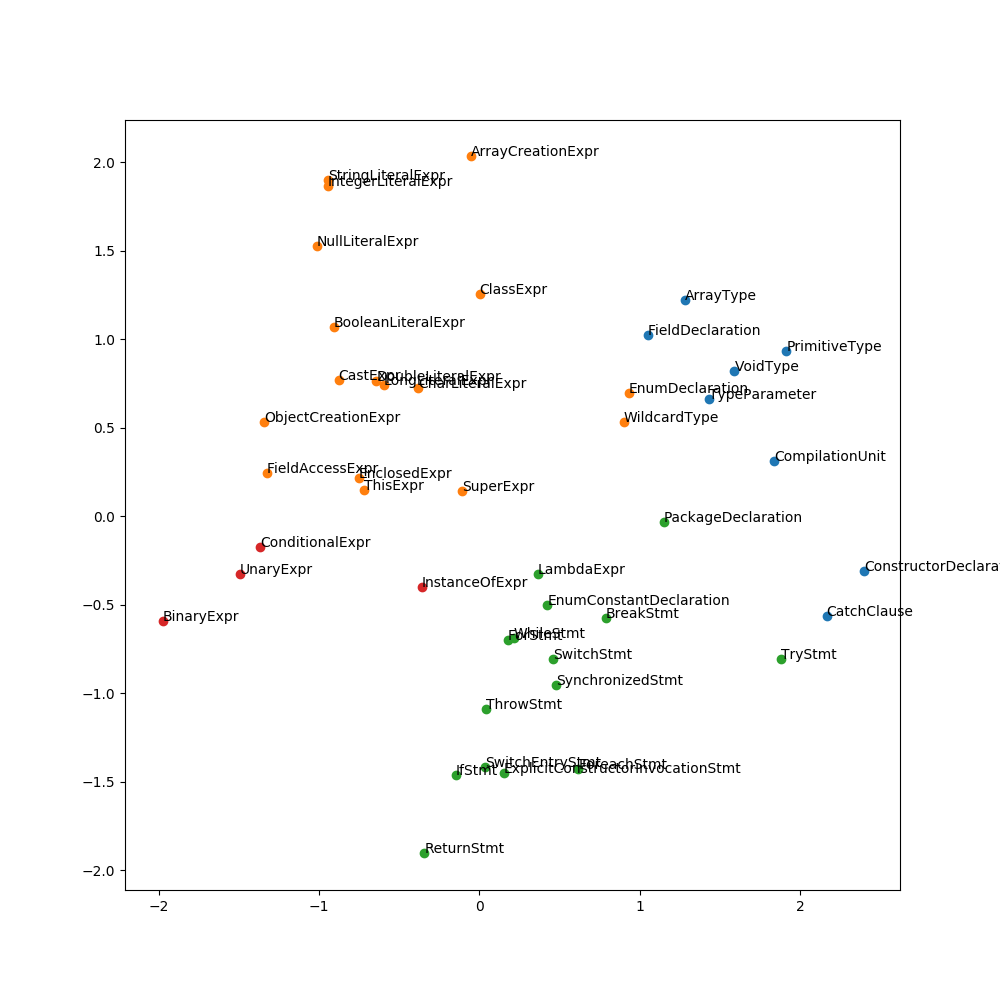
\includegraphics[width=7cm]{../thesis/images/java-embeddings.png}
  \vskip -10mm
  \caption{\label{fig:token-embeddings}Java language level token embeddings}
\end{figure}
\subsection{Clone detection experiments}
Supervised learning approach for cross-language clone detection requires pairs
of code fragments implementing
the same functionality in two different languages.
We choose to generate our dataset from coding competitive programming website,
as they contain a large number of short programs implementing the exact same
functionality. We have scraped all the Python and Java data
from AtCoder\footnote{https://atcoder.jp}. We collected in total about $45000$
code fragments, almost equally balanced between Java and Python, across a set of
about 600 different tasks. We split the dataset in training, cross-validation
and test datasets and run two different types of experiments.

First, we trained our model by providing pairs of code fragments containing
$20$\% of clones to our model --- for each clone pair we feed, we generate $4$
non-clone code pairs and feed them to our model. We train the model to detect
clone between Java and Python and also try to perform Java only clone
detection. We show the results we obtained for both in
tables~\ref{tab:java-python-results} and~\ref{tab:java-java-results} where
``Pretrained'' uses the pretrained embeddings generated
in~\ref{ssec:embedding-generation-experiment} with a vocabulary size of $10000$,
``Untrained'' randomly initializes embeddings instead and ``No identifier'' uses
embeddings generated without token identifiers, yielding a vocabulary of
about $100$ tokens.

\begin{table}
  \caption{\label{tab:java-python-results}Java-Python clone prediction results}
  \centering
  \begin{tabular}{c c c c}
    & F1 & Precision & Recall\\
    \hline%
    Pretrained & $0.66$ & $0.55$ & $0.83$\\
    Untrained & $0.61$ & $0.49$ & $0.82$\\
    No identifier & $0.51$ & $0.40$ & $0.71$
  \end{tabular}
  \vskip -5mm
\end{table}
%
\begin{table}
  \caption{\label{tab:java-java-results}Java-Java clone prediction results}
  \centering
  \begin{tabular}{c c c c}
    & F1 & Precision & Recall\\
    \hline%
    Pretrained & $0.77$ & $0.67$ & $0.92$\\
    Untrained & $0.73$ & $0.65$ & $0.85$\\
    No identifier & $0.69$ & $0.56$ & $0.90$
  \end{tabular}
  \vskip -5mm
\end{table}

Our results show that the model does not perform as well for cross-language
clone detection, which confirms our intuition that it is a harder task than
single-language clone detection. Our pretrained embeddings improve the
performance of our model in both experiments. The performance of our model
decreases when we do not use the identifiers information, but we obtain
reasonable results especially in a single-language context, suggesting than we
do learn information about the code structure.

\begin{table}
  \caption{\label{tab:comparison-results}Comparison with SourecerCC}
  \centering
  \begin{tabular}{c c c c}
    & F1 & Precision & Recall\\
    \hline%
    Our method & $0.21$ & $0.12$ & $0.85$\\
    SourcererCC & $0.05$ & $0.63$ & $0.03$
  \end{tabular}
  \vskip -6mm
\end{table}

In the next experiment, we compare our approach to
SourcererCC~\cite{Sajnani:2016:SSC:2884781.2884877}. We use around $1000$ files,
but as our model can currently only take pairs of code as input, we need to
generate the $n^2$ pairs for $n$ files to test yielding a dataset with a very
low ratio of clones. We suspect that the low precision in
table~\ref{tab:comparison-results} comes from this difference in the data
distribution. However, SourcererCC cannot detect clones on this
data set, with a recall close to $0$, and while our precision is low, we achieve
a high recall meaning that we could at least provide clone candidates.
\section{Future work and conclusion}
We propose a supervised learning approach capable of detecting cross-language
code clones. We also provide a code clone dataset to learn and evaluate a model
using the proposed approach.

In future work, we want to further explore how we can make better use of the
tree structure of the AST when encoding it. We also want to introduce a
hash-layer to our model to be able to index vectors and perform clone detection
in linear time.
\bibliographystyle{ieeetr}
\bibliography{main_bibliography}
\end{document}
